\chapter{Avaliação Experimental}
% explicar objetivos da avaliação experimental.
\section{Ambiente computacional}
Para os experimentos realizados neste trabalho, foram utilizados 2 máquinas com configrações diferentes de hardware. Um deles possui o \textit{hostname} poseidon e é hospedado nas dependências do Laboratório de Arquitetura de Computadores e Microeletrônica (LAM), enquanto o outro trata-se de um notebook pessoal com \textit{hostname} jvdvostro. O servidor poseidon foi utilizado para realizar a busca de hiperparâmetros, pois é a etapa que mais consome recursos computacionais. O jvdvostro foi utilizado para coletar as métricas de inferência, gerar gráficos e fazer a análise dos resultados. A Tabela~\ref{tab:hardware} expõe as configurações de \textit{hardware} de ambos computadores utilizados nos experimentos.

\begin{table}[!htp]\centering \label{tab:hardware}
    \caption{Configurações de \textit{hardware} dos computadores}
    \begin{tabular}{lrrrrr}\toprule
    \end{tabular}
\end{table}

Os experimentos foram realizados utilizando \textit{scripts} e \textit{notebooks} Python, dependendo da etapa e da finalidade. Para a busca de hiperparâmetros e avaliação dos modelos em relação ao erro, foram utilizados \textit{scripts}, enquanto para a avaliação de métricas de tempo de inferência e uso de memória foram utilizados \textit{notebooks}.

\section{Coleções de dados}
Foram utilizadas para os experimentos deste trabalho 3 coleções de dados. Dentre estas, duas foram coletadas de fontes públicas abertas na internet e uma foi gerada artificialmente. Todas foram armazenadas em disco local no formato tabular com extensão CSV. O número de casos confirmados de Covid19 no Rio de Janeiro foi o primeiro dataset utilizado nos experimentos e serviu um dos motivadores do estudo realizado. A temperatura mínima diária em Melbourne e os dados gerados sintéticamente serviram como prova de conceito para averiguar a eficiência dos métodos aplicados em diferentes cenários, portanto foram submetidos aos mesmos métodos e técnicas aplicados na primeira coleção de dados.

\subsection{Casos confirmados de Covid19 no Rio de Janeiro}
Com o auxílio da biblioteca \textit{requests} do Python, foi criado um script para baixar e armazenar localmente o número de casos confirmados de Covid19 no Estado do Rio de Janeiro. O arquivo csv foi baixado diretamente do web site da Secretaria de Saúde do Estado do Rio de Janeiro. \footnote{$http://sistemas.saude.rj.gov.br/tabnetbd/dhx.exe?covid19/covid_munic_diario.def$} Para manter a reprodutibilidade dos experimentos, o período analisado foi congelado entre as datas 01/01/2020 e 04/07/2021. A Figura~\ref{fig:casos_confirmados} mostra um gráfico da série temporal não acumulada do número de casos confirmados diário, ou seja, os valores absolutos de casos registrados em cada dia sem considerar os dias anteriores.

\begin{figure}[!htp] \label{fig:casos_confirmados}
    \centering
    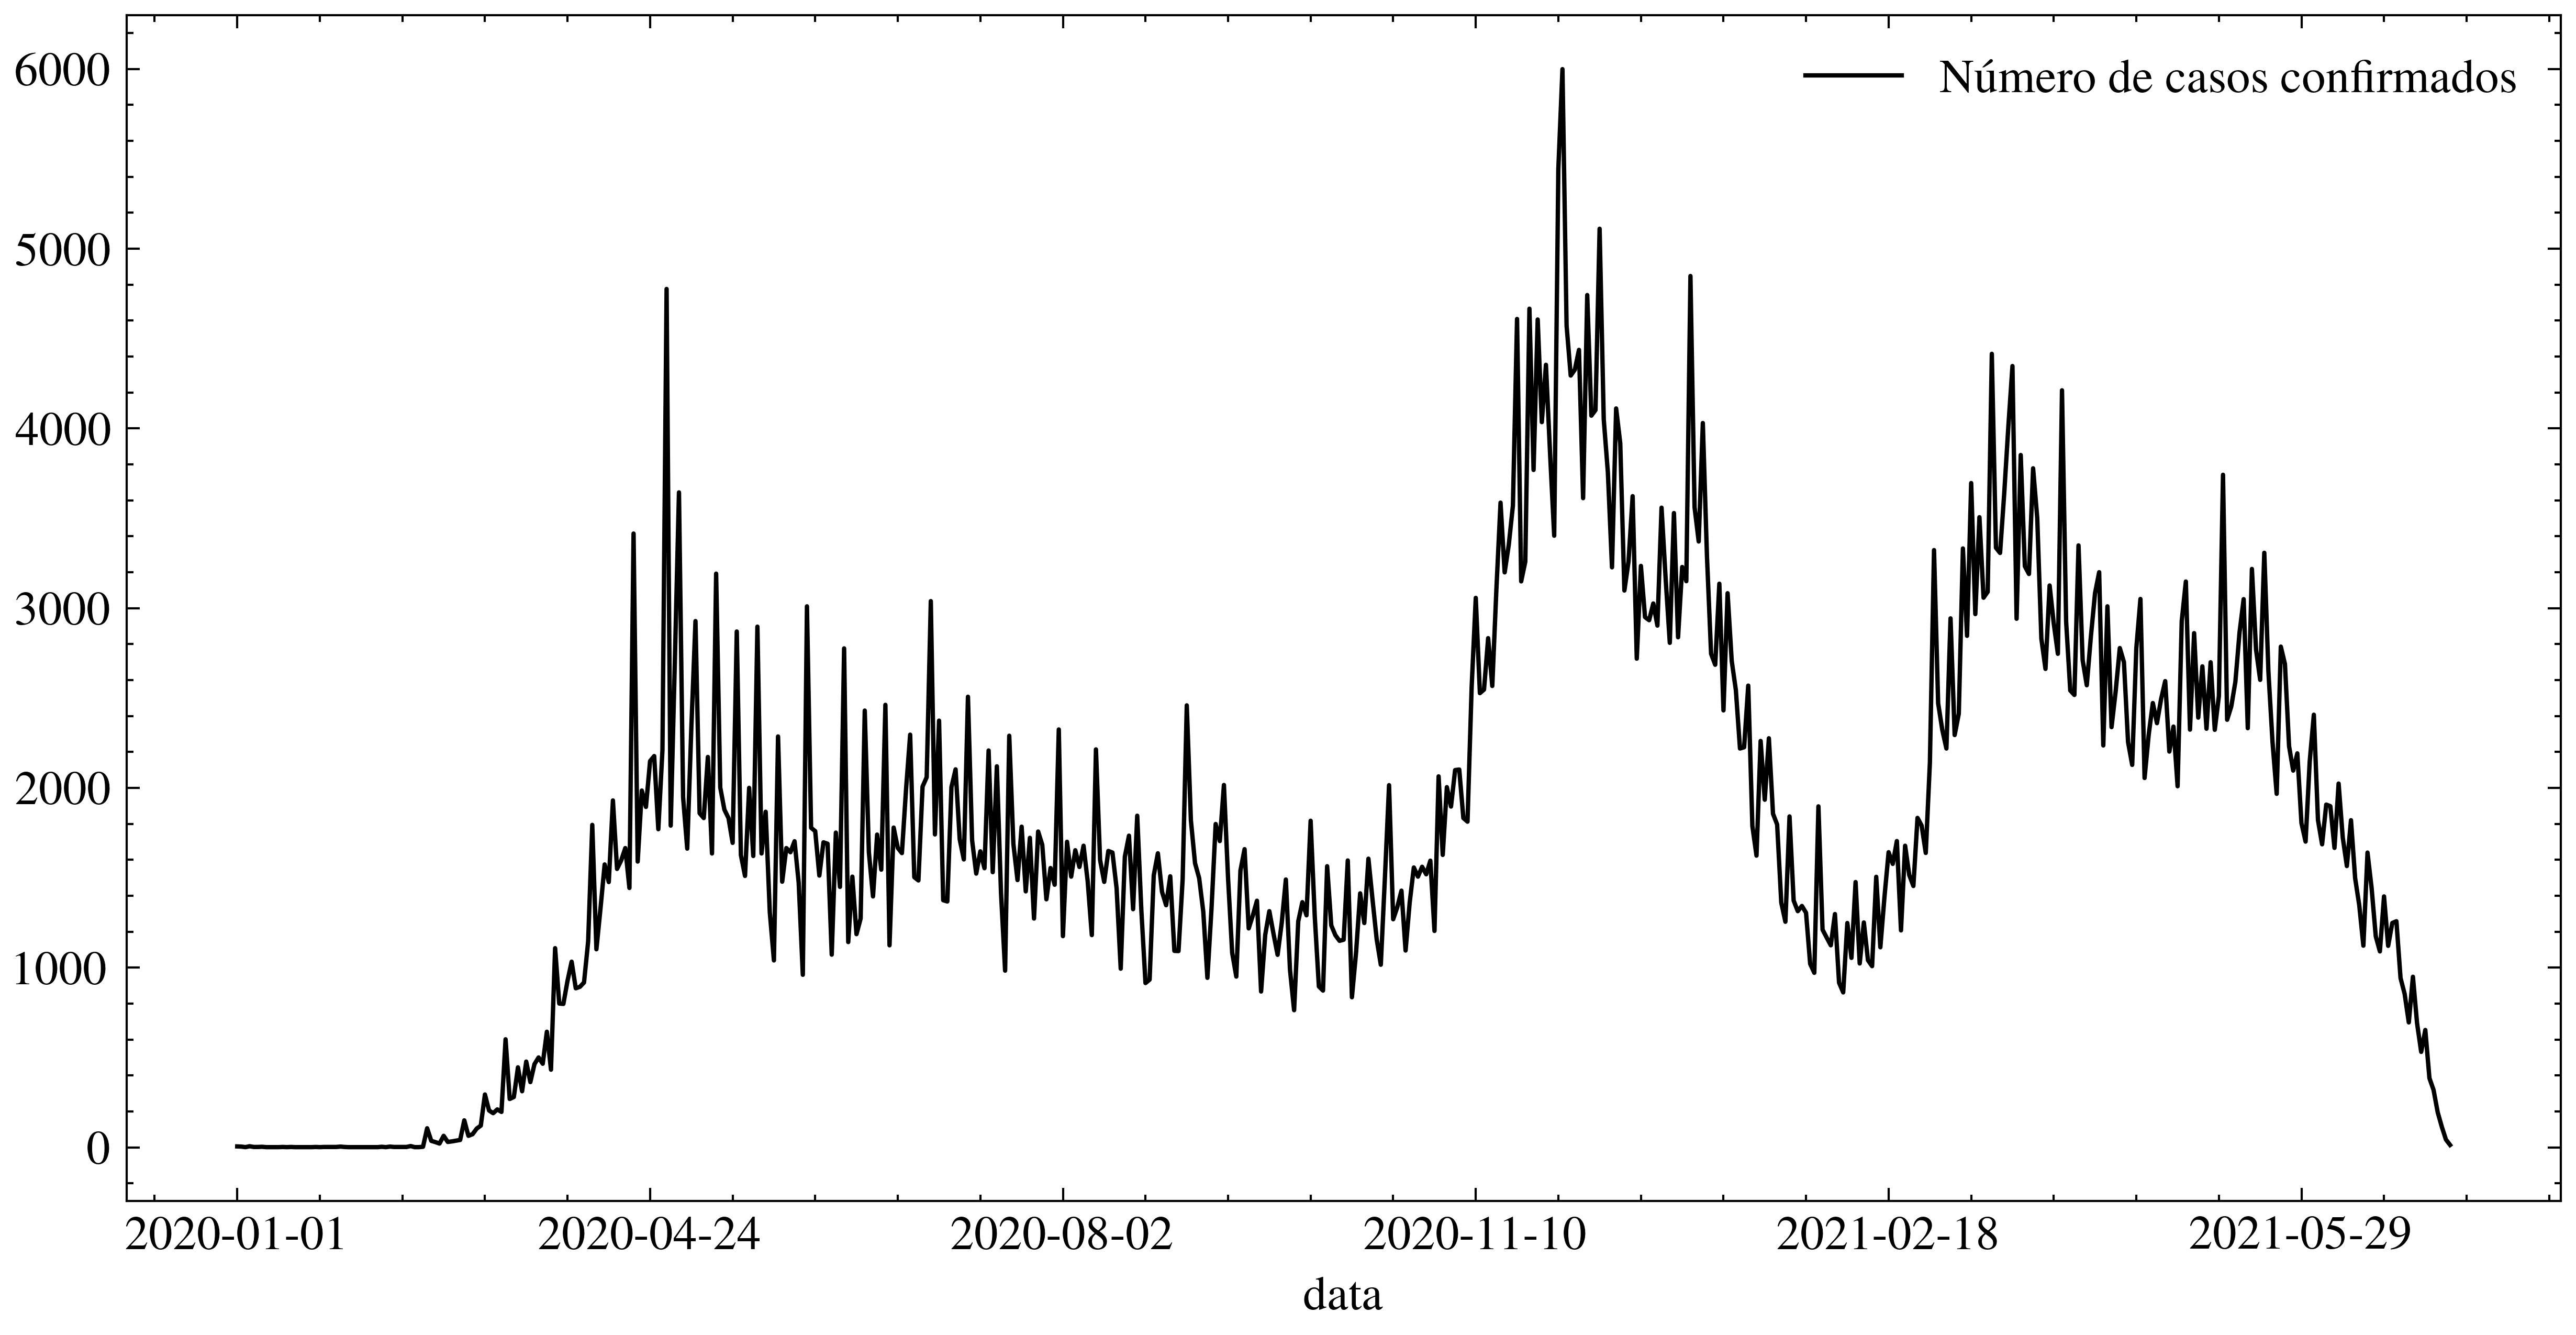
\includegraphics[width=5.0in]{img/casos_confirmados.png}
    \caption{Série temporal de casos confirmados de Covid19 no Rio de Janeiro}
\end{figure}

A Figura~\ref{fig:casos_confirmados} mostra que há flutuações a curto pazo, que podem ter sido geradas por diversos fatores na coleta dos dados, como, por exemplo, a subamostragem. Como a coleta dos dados utilizados foi feita de fontes externas e públicas, os experimentos deste se limitaram a trabalhar com o dado como foi disponibilizado, sem aprofundar na avaliação da coleta. Porém, para remover a influência dessas flutuações, foi aplicado o método de médias móveis variando o parâmetro do número de amostras junto à busca de hiperparâmetros para encontrar o melhor ajuste. A Figura~\ref{fig:medias_moveis} mostra a mesma série temporal com as médias móveis em vermelho considerando-se o parâmetro $n=7$ como exemplo de suavização na flutuação dos valores da série temporal.

\begin{figure}[!htp] \label{fig:medias_moveis}
    \centering
    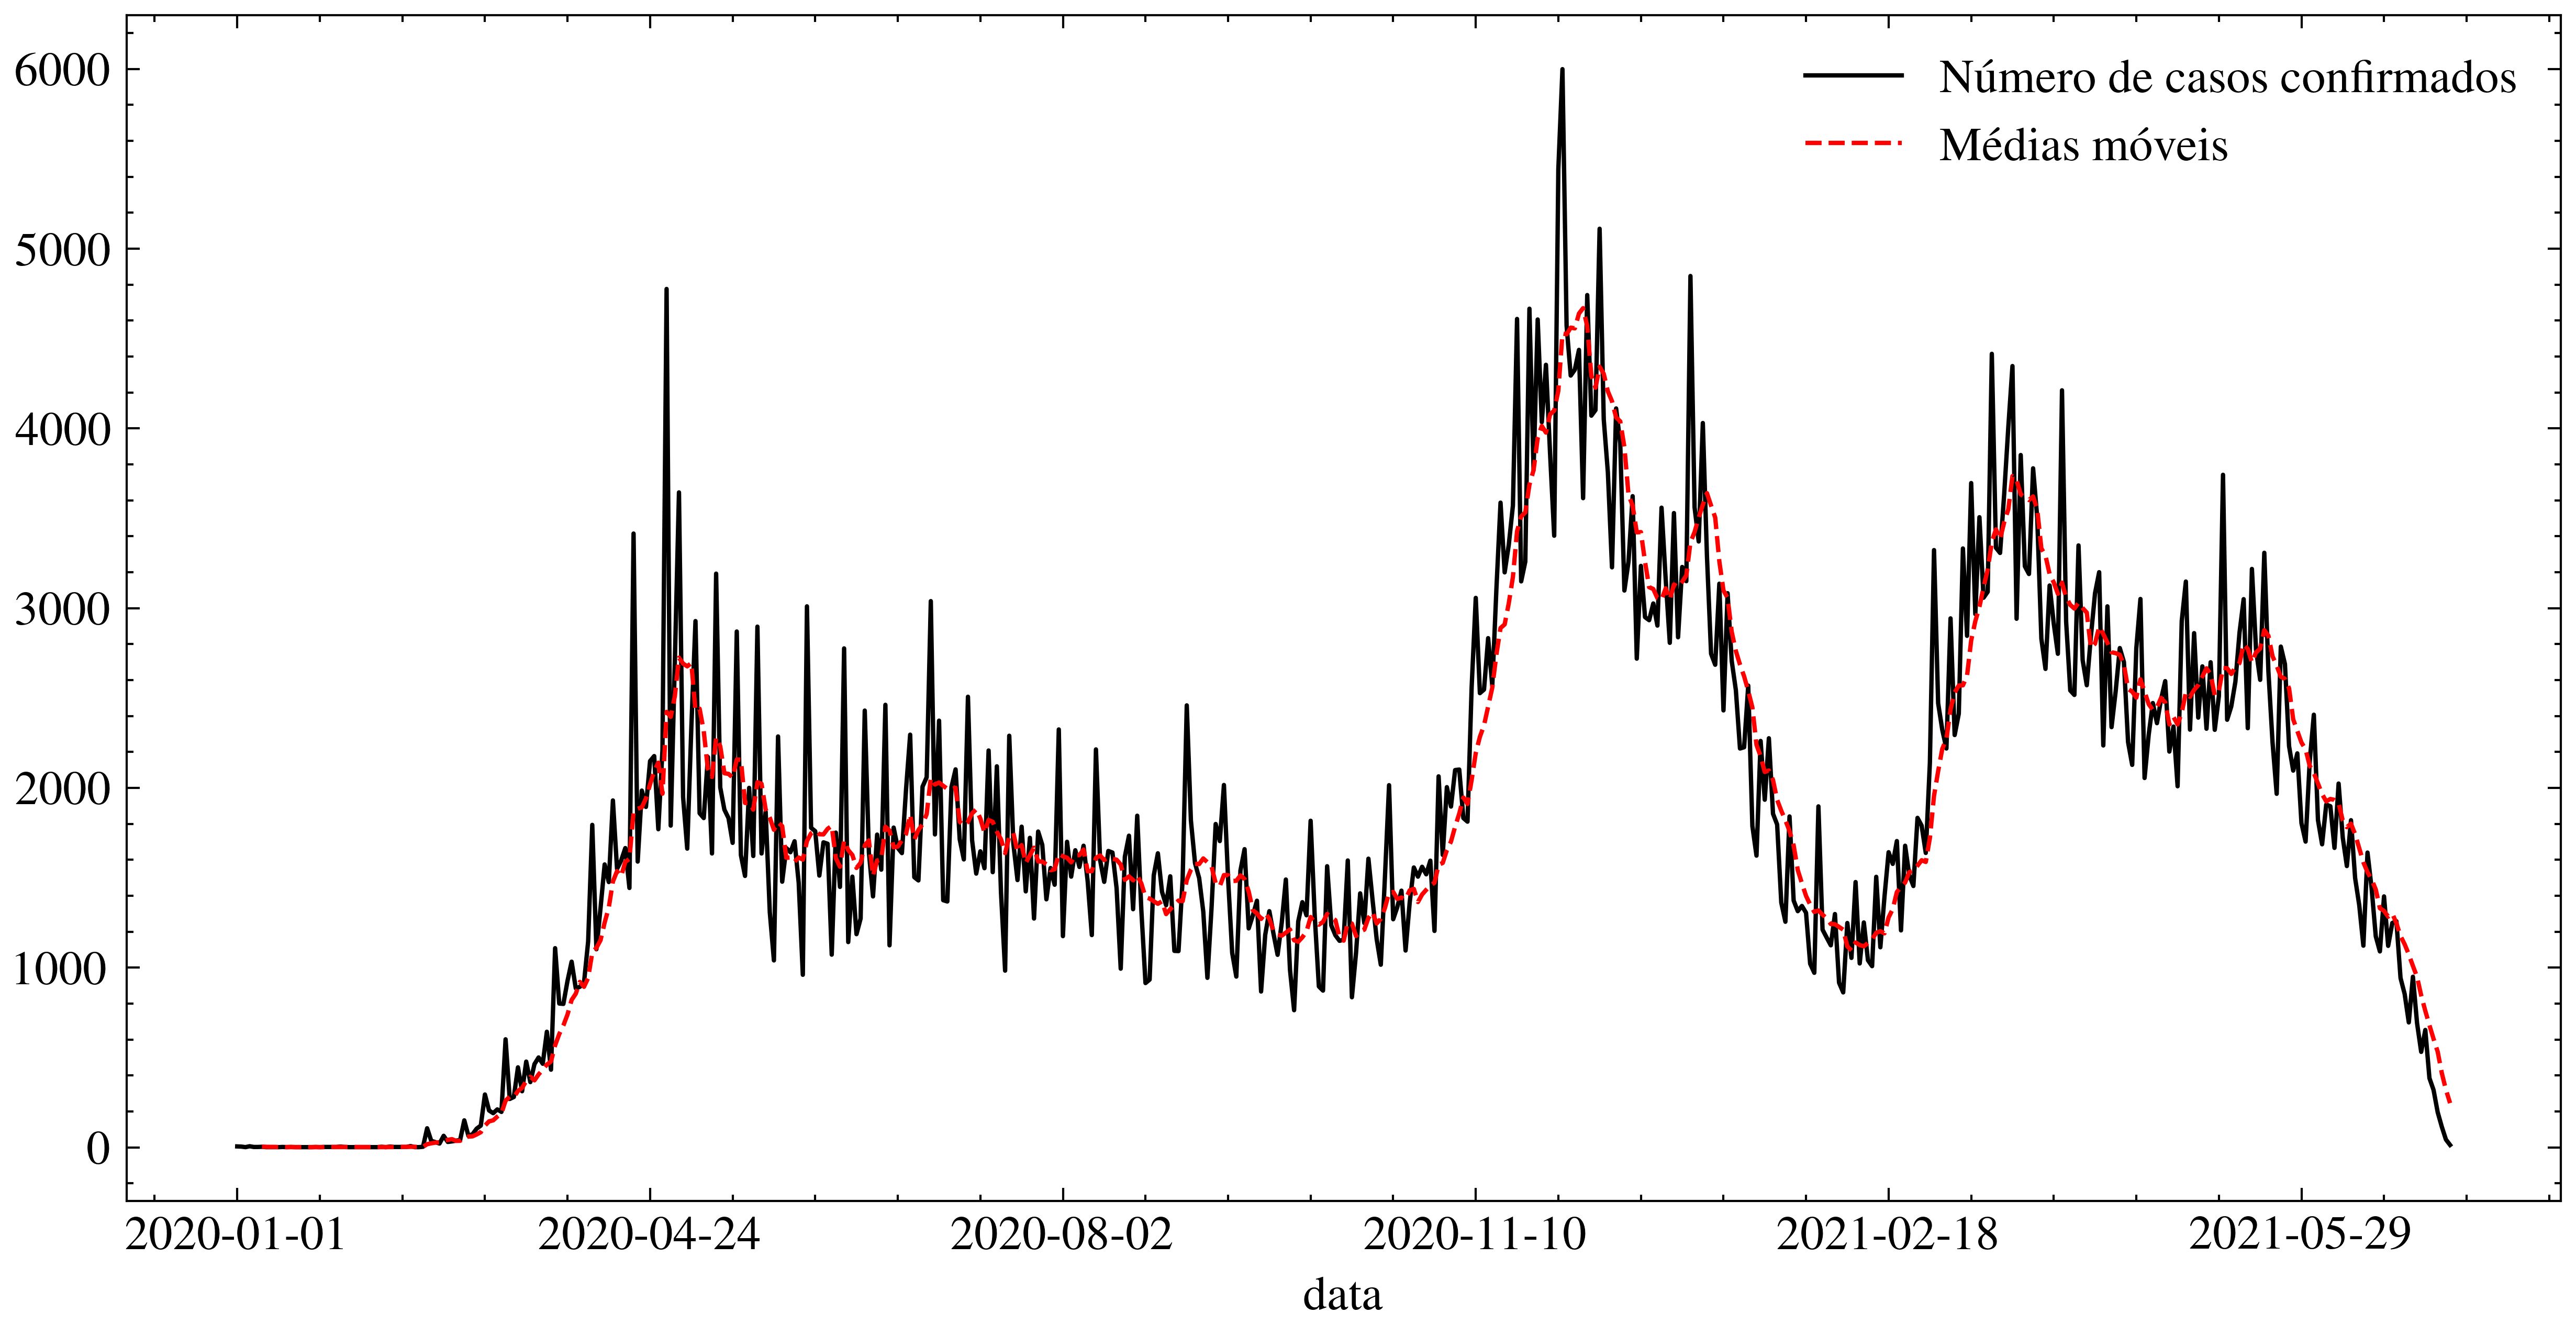
\includegraphics[width=5.0in]{img/medias_moveis.png}
    \caption{Médias móveis da série temporal de casos confirmados de Covid19 no Rio de Janeiro}
\end{figure}

\subsection{Temperatura mínima diária em Melbourne}

\subsection{Série temporal sintética}
Uma coleção de dados foi gerada de forma sintética com o auxílio da biblioteca \textit{numpy} do Python com características criadas artificialmente somando componentes como tendência, sazonalidade, ruído branco e fatores para distorção da estacionaridade.

\section{Métricas de avaliação utilizadas}

\section{Resultados}
% apresentar formato de apresentação dos resultados.

\subsection{Avaliação por métricas}

\subsection{Tempos de execução}

\begin{table}[!htp]
    \caption{Tempo de ajuste dos modelos}
    \begin{tabular}{|c|c|ccc|}
        \hline
        \rowcolor[HTML]{C0C0C0}
        \cellcolor[HTML]{C0C0C0}                          & \cellcolor[HTML]{C0C0C0}                          & \multicolumn{3}{c|}{\cellcolor[HTML]{C0C0C0}Dataset}                                                                                                                         \\ \cline{3-5}
        \rowcolor[HTML]{C0C0C0}
        \multirow{-2}{*}{\cellcolor[HTML]{C0C0C0}Modelo}  & \multirow{-2}{*}{\cellcolor[HTML]{C0C0C0}Métrica} & \multicolumn{1}{c|}{\cellcolor[HTML]{C0C0C0}Covid}                      & \multicolumn{1}{c|}{\cellcolor[HTML]{C0C0C0}Temperatura}               & Sintético                 \\ \hline
        \cellcolor[HTML]{C0C0C0}                          & RMSE                                              & \multicolumn{1}{c|}{779 ms ± 2.4 ms}                                    & \multicolumn{1}{c|}{3.61 s ± 5.34 ms}                                  & 38.4 ms ± 383 µs          \\ \cline{2-5}
        \rowcolor[HTML]{EFEFEF}
        \cellcolor[HTML]{C0C0C0}                          & MAPE                                              & \multicolumn{1}{c|}{\cellcolor[HTML]{EFEFEF}1.34 s ± 2.11ms}            & \multicolumn{1}{c|}{\cellcolor[HTML]{EFEFEF}3.61 s ± 4.68 ms}          & 38.3 ms ± 184 µs          \\ \cline{2-5}
        \cellcolor[HTML]{C0C0C0}                          & MAE                                               & \multicolumn{1}{c|}{779 ms ± 1.2 ms}                                    & \multicolumn{1}{c|}{3.61 s ± 8.5 ms}                                   & 38.4 ms ± 225 µs          \\ \cline{2-5}
        \rowcolor[HTML]{EFEFEF}
        \multirow{-4}{*}{\cellcolor[HTML]{C0C0C0}ARIMA}   & MPE                                               & \multicolumn{1}{c|}{\cellcolor[HTML]{EFEFEF}1.61 s ± 1.33 ms}           & \multicolumn{1}{c|}{\cellcolor[HTML]{EFEFEF}6.36 s ± 9.48 ms}          & 566 ms ± 705 µs           \\ \hline
        \cellcolor[HTML]{C0C0C0}                          & RMSE                                              & \multicolumn{1}{c|}{\textbf{4.41 ms ± 151 µs}}                          & \multicolumn{1}{c|}{\textbf{31.2 ms ± 526 µs}}                         & \textbf{9.97 ms ± 143 µs} \\ \cline{2-5}
        \rowcolor[HTML]{EFEFEF}
        \cellcolor[HTML]{C0C0C0}                          & MAPE                                              & \multicolumn{1}{c|}{\cellcolor[HTML]{EFEFEF}\textbf{4.46 ms ± 75.1 µs}} & \multicolumn{1}{c|}{\cellcolor[HTML]{EFEFEF}\textbf{19.5 ms ± 409 µs}} & \textbf{10.1 ms ± 166 µs} \\ \cline{2-5}
        \cellcolor[HTML]{C0C0C0}                          & MAE                                               & \multicolumn{1}{c|}{\textbf{8.65 ms ± 126 µs}}                          & \multicolumn{1}{c|}{\textbf{19.3 ms ± 149 µs}}                         & \textbf{10.5 ms ± 116 µs} \\ \cline{2-5}
        \rowcolor[HTML]{EFEFEF}
        \multirow{-4}{*}{\cellcolor[HTML]{C0C0C0}ReW}     & MPE                                               & \multicolumn{1}{c|}{\cellcolor[HTML]{EFEFEF}\textbf{4.41 ms ± 151 µs}}  & \multicolumn{1}{c|}{\cellcolor[HTML]{EFEFEF}\textbf{64.7 ms ± 549 µs}} & \textbf{8.86 ms ± 123 µs} \\ \hline
        \cellcolor[HTML]{C0C0C0}                          & RMSE                                              & \multicolumn{1}{c|}{56.5 ms ± 17.9 ms}                                  & \multicolumn{1}{c|}{205 ms ± 176 µs}                                   & 60.7 ms ± 87 µs           \\ \cline{2-5}
        \rowcolor[HTML]{EFEFEF}
        \cellcolor[HTML]{C0C0C0}                          & MAPE                                              & \multicolumn{1}{c|}{\cellcolor[HTML]{EFEFEF}46 ms ± 63.1 µs}            & \multicolumn{1}{c|}{\cellcolor[HTML]{EFEFEF}179 ms ± 514 µs}           & 60.9 ms ± 174 µs          \\ \cline{2-5}
        \cellcolor[HTML]{C0C0C0}                          & MAE                                               & \multicolumn{1}{c|}{44.6 ms ± 109 µs}                                   & \multicolumn{1}{c|}{180 ms ± 396 µs}                                   & 61.1 ms ± 177 µs          \\ \cline{2-5}
        \rowcolor[HTML]{EFEFEF}
        \multirow{-4}{*}{\cellcolor[HTML]{C0C0C0}Prophet} & MPE                                               & \multicolumn{1}{c|}{\cellcolor[HTML]{EFEFEF}46 ms ± 72.1 µs}            & \multicolumn{1}{c|}{\cellcolor[HTML]{EFEFEF}203 ms ± 200 µs}           & 68.1 ms ± 178 µs          \\ \hline
    \end{tabular}
\end{table}

\begin{table}[!htp]
    \caption{Tempo de inferência dos modelos}
    \begin{tabular}{|c|c|ccc|}
        \hline
        \rowcolor[HTML]{C0C0C0}
        \cellcolor[HTML]{C0C0C0}                          & \cellcolor[HTML]{C0C0C0}                          & \multicolumn{3}{c|}{\cellcolor[HTML]{C0C0C0}Dataset}                                                                                                                         \\ \cline{3-5}
        \rowcolor[HTML]{C0C0C0}
        \multirow{-2}{*}{\cellcolor[HTML]{C0C0C0}Modelo}  & \multirow{-2}{*}{\cellcolor[HTML]{C0C0C0}Métrica} & \multicolumn{1}{c|}{\cellcolor[HTML]{C0C0C0}Covid}                      & \multicolumn{1}{c|}{\cellcolor[HTML]{C0C0C0}Temperatura}               & Sintético                 \\ \hline
        \cellcolor[HTML]{C0C0C0}                          & RMSE                                              & \multicolumn{1}{c|}{960 µs ± 2.51 µs}                                   & \multicolumn{1}{c|}{951 µs ± 14.4 µs}                                  & 1.92 ms ± 28.5 µs         \\ \cline{2-5}
        \rowcolor[HTML]{EFEFEF}
        \cellcolor[HTML]{C0C0C0}                          & MAPE                                              & \multicolumn{1}{c|}{\cellcolor[HTML]{EFEFEF}970 µs ± 1.83 µs}           & \multicolumn{1}{c|}{\cellcolor[HTML]{EFEFEF}942 µs ± 4.96 µs}          & 1.93 ms ± 33.3 µs         \\ \cline{2-5}
        \cellcolor[HTML]{C0C0C0}                          & MAE                                               & \multicolumn{1}{c|}{958 µs ± 2.81 µs}                                   & \multicolumn{1}{c|}{972 µs ± 8.09 µs}                                  & 1.92 ms ± 24.8 µs         \\ \cline{2-5}
        \rowcolor[HTML]{EFEFEF}
        \multirow{-4}{*}{\cellcolor[HTML]{C0C0C0}ARIMA}   & MPE                                               & \multicolumn{1}{c|}{\cellcolor[HTML]{EFEFEF}959 µs ± 5.72 µs}           & \multicolumn{1}{c|}{\cellcolor[HTML]{EFEFEF}956 µs ± 7.02 µs}          & 953 µs ± 27.8 µs          \\ \hline
        \cellcolor[HTML]{C0C0C0}                          & RMSE                                              & \multicolumn{1}{c|}{\textbf{142 µs ± 2.8 µs}}                           & \multicolumn{1}{c|}{\textbf{149 µs ± 349 ns}}                          & \textbf{330 µs ± 4.67}    \\ \cline{2-5}
        \rowcolor[HTML]{EFEFEF}
        \cellcolor[HTML]{C0C0C0}                          & MAPE                                              & \multicolumn{1}{c|}{\cellcolor[HTML]{EFEFEF}\textbf{87.6 µs ± 1.22 µs}} & \multicolumn{1}{c|}{\cellcolor[HTML]{EFEFEF}\textbf{106 µs ± 339 ns}}  & \textbf{494 µs ± 12.8 µs} \\ \cline{2-5}
        \cellcolor[HTML]{C0C0C0}                          & MAE                                               & \multicolumn{1}{c|}{\textbf{145 µs ± 2.3 µs}}                           & \multicolumn{1}{c|}{\textbf{107 µs ± 1.45 µs}}                         & \textbf{512 µs ± 7.91 µs} \\ \cline{2-5}
        \rowcolor[HTML]{EFEFEF}
        \multirow{-4}{*}{\cellcolor[HTML]{C0C0C0}ReW}     & MPE                                               & \multicolumn{1}{c|}{\cellcolor[HTML]{EFEFEF}\textbf{91 µs ± 638 ns}}    & \multicolumn{1}{c|}{\cellcolor[HTML]{EFEFEF}\textbf{232 µs ± 6.43 µs}} & \textbf{422 µs ± 8.16 µs} \\ \hline
        \cellcolor[HTML]{C0C0C0}                          & RMSE                                              & \multicolumn{1}{c|}{1.26 s ± 10.7 ms}                                   & \multicolumn{1}{c|}{1.88 s ± 3.79 ms}                                  & 898 ms ± 768 µs           \\ \cline{2-5}
        \rowcolor[HTML]{EFEFEF}
        \cellcolor[HTML]{C0C0C0}                          & MAPE                                              & \multicolumn{1}{c|}{\cellcolor[HTML]{EFEFEF}1.25 s ± 1.59 ms}           & \multicolumn{1}{c|}{\cellcolor[HTML]{EFEFEF}2.13 s ± 711 µs}           & 906 ms ± 600 µs           \\ \cline{2-5}
        \cellcolor[HTML]{C0C0C0}                          & MAE                                               & \multicolumn{1}{c|}{1.25 s ± 1.29 ms}                                   & \multicolumn{1}{c|}{2.13 s ± 940 µs}                                   & 898 ms ± 753 µs           \\ \cline{2-5}
        \rowcolor[HTML]{EFEFEF}
        \multirow{-4}{*}{\cellcolor[HTML]{C0C0C0}Prophet} & MPE                                               & \multicolumn{1}{c|}{\cellcolor[HTML]{EFEFEF}1.25 s ± 1.26 ms}           & \multicolumn{1}{c|}{\cellcolor[HTML]{EFEFEF}1.88 s ± 530 µs}           & 899 ms ± 1.24 ms          \\ \hline
    \end{tabular}
\end{table}

\subsection{Uso de memória}

\begin{table}[!htp]
    \caption{Uso de memória de cada modelo por métrica otimizada e dataset}
    \centering
    \begin{tabular}{|c|c|ccc|}
        \hline
        \rowcolor[HTML]{C0C0C0}
        \cellcolor[HTML]{C0C0C0}                          & \cellcolor[HTML]{C0C0C0}                          & \multicolumn{3}{c|}{\cellcolor[HTML]{C0C0C0}Dataset}                                                                                                   \\ \cline{3-5}
        \rowcolor[HTML]{C0C0C0}
        \multirow{-2}{*}{\cellcolor[HTML]{C0C0C0}Modelo}  & \multirow{-2}{*}{\cellcolor[HTML]{C0C0C0}Métrica} & \multicolumn{1}{c|}{\cellcolor[HTML]{C0C0C0}Covid}              & \multicolumn{1}{c|}{\cellcolor[HTML]{C0C0C0}Temperatura}        & Sintético          \\ \hline
        \cellcolor[HTML]{C0C0C0}                          & RMSE                                              & \multicolumn{1}{c|}{9.086 MiB}                                  & \multicolumn{1}{c|}{43.621 MiB}                                 & 3.105 MiB          \\ \cline{2-5}
        \rowcolor[HTML]{EFEFEF}
        \cellcolor[HTML]{C0C0C0}                          & MAPE                                              & \multicolumn{1}{c|}{\cellcolor[HTML]{EFEFEF}11.383 MiB}         & \multicolumn{1}{c|}{\cellcolor[HTML]{EFEFEF}43.699 MiB}         & 3.078 MiB          \\ \cline{2-5}
        \cellcolor[HTML]{C0C0C0}                          & MAE                                               & \multicolumn{1}{c|}{8.816 MiB}                                  & \multicolumn{1}{c|}{44.035 MiB}                                 & 3.359 MiB          \\ \cline{2-5}
        \rowcolor[HTML]{EFEFEF}
        \multirow{-4}{*}{\cellcolor[HTML]{C0C0C0}ARIMA}   & MPE                                               & \multicolumn{1}{c|}{\cellcolor[HTML]{EFEFEF}13.734 MiB}         & \multicolumn{1}{c|}{\cellcolor[HTML]{EFEFEF}50.805 MiB}         & 6.457 MiB          \\ \hline
        \cellcolor[HTML]{C0C0C0}                          & RMSE                                              & \multicolumn{1}{c|}{\textbf{0.512 MiB}}                         & \multicolumn{1}{c|}{\textbf{1.039 MiB}}                         & \textbf{0.598 MiB} \\ \cline{2-5}
        \rowcolor[HTML]{EFEFEF}
        \cellcolor[HTML]{C0C0C0}                          & MAPE                                              & \multicolumn{1}{c|}{\cellcolor[HTML]{EFEFEF}\textbf{0.000 MiB}} & \multicolumn{1}{c|}{\cellcolor[HTML]{EFEFEF}\textbf{0.922 MiB}} & \textbf{0.570 MiB} \\ \cline{2-5}
        \cellcolor[HTML]{C0C0C0}                          & MAE                                               & \multicolumn{1}{c|}{\textbf{0.586 MiB}}                         & \multicolumn{1}{c|}{\textbf{0.887 MiB}}                         & \textbf{0.898 MiB} \\ \cline{2-5}
        \rowcolor[HTML]{EFEFEF}
        \multirow{-4}{*}{\cellcolor[HTML]{C0C0C0}ReW}     & MPE                                               & \multicolumn{1}{c|}{\cellcolor[HTML]{EFEFEF}\textbf{0.645 MiB}} & \multicolumn{1}{c|}{\cellcolor[HTML]{EFEFEF}\textbf{0.809 MiB}} & \textbf{0.562 MiB} \\ \hline
        \cellcolor[HTML]{C0C0C0}                          & RMSE                                              & \multicolumn{1}{c|}{90.676 MiB}                                 & \multicolumn{1}{c|}{101.699 MiB}                                & 89.719 MiB         \\ \cline{2-5}
        \rowcolor[HTML]{EFEFEF}
        \cellcolor[HTML]{C0C0C0}                          & MAPE                                              & \multicolumn{1}{c|}{\cellcolor[HTML]{EFEFEF}90.652 MiB}         & \multicolumn{1}{c|}{\cellcolor[HTML]{EFEFEF}102.074 MiB}        & 89.203 MiB         \\ \cline{2-5}
        \cellcolor[HTML]{C0C0C0}                          & MAE                                               & \multicolumn{1}{c|}{90.621 MiB}                                 & \multicolumn{1}{c|}{102.273 MiB}                                & 89.426 MiB         \\ \cline{2-5}
        \rowcolor[HTML]{EFEFEF}
        \multirow{-4}{*}{\cellcolor[HTML]{C0C0C0}Prophet} & MPE                                               & \multicolumn{1}{c|}{\cellcolor[HTML]{EFEFEF}90.617 MiB}         & \multicolumn{1}{c|}{\cellcolor[HTML]{EFEFEF}101.926 MiB}        & 89.277 MiB         \\ \hline
    \end{tabular}
\end{table}
\subsection{Discussão}
